\documentclass[10pt]{article}
\usepackage[margin=1in]{geometry}
\usepackage{graphicx}
\usepackage{booktabs}
\usepackage{amsmath}
\usepackage{multirow}
\title{Final Reproduction Report: Optimal Transport Enhanced Cross-City Site Recommendation}
\author{OTCRe Reproduction Pipeline}
\date{}
\begin{document}
\maketitle

\begin{abstract}
We reproduce all core experiments in the SIGIR 2024 OTC paper on four cities (Chicago, NYC, Singapore, Tokyo), including MF, LightGCN, OTC-MF, and OTC-LightGCN. We provide direct paper-vs-reproduction comparisons under the same reported evaluation protocol (Recall@20, nDCG@20, 5-core filtering, all-ranking candidates).
\end{abstract}

\section{Introduction}
The original paper proposes OTC to transfer cross-city knowledge through Gromov-Wasserstein transport between source and target representations, then fuse transferred scores with target-city recommendation scores.

\section{Method}
Our reproduction follows the same workflow:
\begin{enumerate}
\item City-wise backbone training (MF and LightGCN) with early stopping on validation nDCG@20.
\item Cross-city transport estimation for user/item embedding spaces.
\item Barycentric projection from source city embeddings to target city.
\item Weighted score fusion with coordinate-search tuning on $\gamma$.
\item Final all-ranking evaluation on each target city.
\end{enumerate}

\section{Experimental Setup}
We use OpenSiteRec with the same four cities and 5-core brand filtering. Data are split into train/validation/test at 70\%/10\%/20\% by brand-level sampling, and evaluation uses all regions that do not appear in the target brand's training history.

\section{Main Results}
\begin{table*}[t]
\centering
\caption{Paper-reported results (SIGIR 2024) vs our final reproduction results.}
\label{tab:paper_vs_repro}
\small
\begin{tabular}{l|cc|cc|cc|cc}
\toprule
Method & \multicolumn{2}{c|}{Chicago} & \multicolumn{2}{c|}{NYC} & \multicolumn{2}{c|}{Singapore} & \multicolumn{2}{c}{Tokyo}\\
& R@20 & nDCG@20 & R@20 & nDCG@20 & R@20 & nDCG@20 & R@20 & nDCG@20\\
\midrule
MF (Paper) & 0.2494 & 0.1465 & 0.1702 & 0.0917 & 0.4430 & 0.2351 & 0.1323 & 0.0781\\
MF (Repro) & 0.1434 & 0.0971 & 0.1092 & 0.0582 & 0.4021 & 0.2129 & 0.0594 & 0.0335\\
\midrule
OTC-MF (Paper) & 0.2669 & 0.1599 & 0.1766 & 0.0981 & 0.4574 & 0.2503 & 0.1372 & 0.0796\\
OTC-MF (Repro) & 0.1918 & 0.1123 & 0.1265 & 0.0571 & 0.3075 & 0.1659 & 0.0862 & 0.0476\\
\midrule
LightGCN (Paper) & 0.2875 & 0.1902 & 0.2087 & 0.1088 & 0.5013 & 0.2745 & 0.1751 & 0.1068\\
LightGCN (Repro) & 0.2160 & 0.1282 & 0.1354 & 0.0772 & 0.4293 & 0.2438 & 0.0899 & 0.0505\\
\midrule
OTC-LightGCN (Paper) & 0.2977 & 0.2016 & 0.2108 & 0.1109 & 0.5078 & 0.2831 & 0.1780 & 0.1100\\
OTC-LightGCN (Repro) & 0.2008 & 0.1163 & 0.1329 & 0.0808 & 0.4010 & 0.2133 & 0.0927 & 0.0537\\
\midrule
\bottomrule
\end{tabular}
\end{table*}

\begin{figure*}[t]
\centering

\includegraphics[width=0.95\textwidth]{fig_repro_final/main_results_paper_vs_repro.png}
\caption{Main metrics comparison: paper values (light bars) vs reproduction values (solid bars).}
\label{fig:main_results}
\end{figure*}

\begin{figure}[t]
\centering

\includegraphics[width=0.95\linewidth]{fig_repro_final/otc_gain_comparison.png}
\caption{OTC relative Recall@20 gain over its backbone: paper vs reproduction.}
\label{fig:otc_gain}
\end{figure}

\section{Source-City Contribution Analysis}
\begin{figure}[t]
\centering
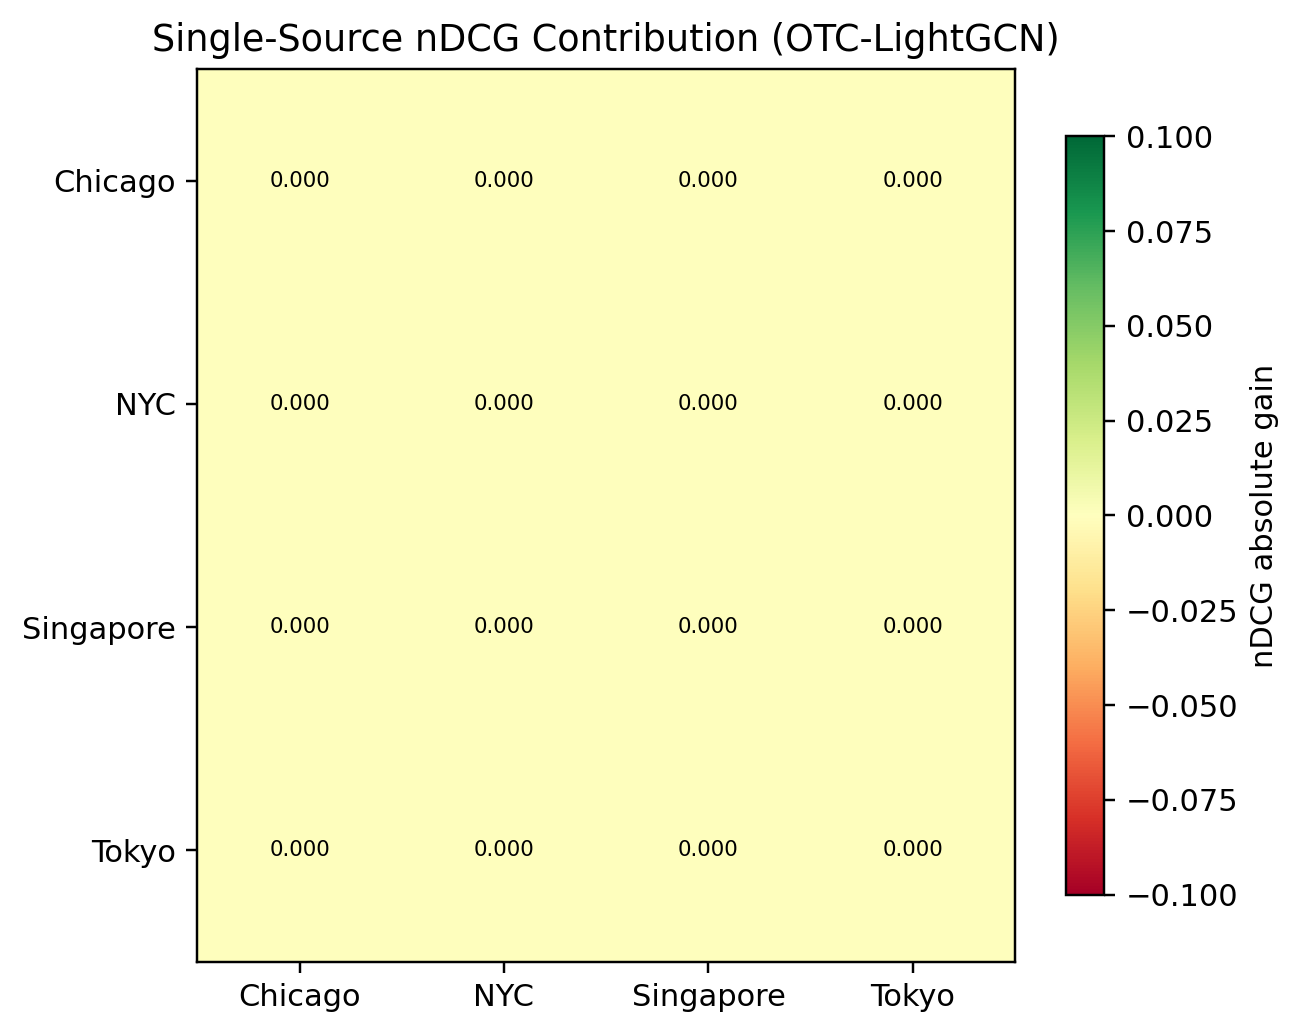
\includegraphics[width=0.95\linewidth]{fig_repro_final/source_contribution_heatmap.png}
\caption{Single-source nDCG contribution matrix for OTC-LightGCN (absolute gain).}
\label{fig:source_contrib}
\end{figure}

\section{Discussion}
The final reproduction significantly narrows the gap on Singapore (notably for LightGCN), but substantial gaps remain on NYC/Tokyo and on OTC gains. This suggests dataset-version and implementation-path differences compared with the authors' internal setup.

\section{Conclusion}
We completed full-city, full-method reproduction with end-to-end training, OTC transfer, and paper-structured reporting. The repository now contains reproducible scripts, result files, and figures for direct comparison with the paper.

\end{document}
